%  article.tex (Version 3.3, released 19 January 2008)
%  Article to demonstrate format for SPIE Proceedings
%  Special instructions are included in this file after the
%  symbol %>>>>
%  Numerous commands are commented out, but included to show how
%  to effect various options, e.g., to print page numbers, etc.
%  This LaTeX source file is composed for LaTeX2e.

%  The following commands have been added in the SPIE class 
%  file (spie.cls) and will not be understood in other classes:
%  \supit{}, \authorinfo{}, \skiplinehalf, \keywords{}
%  The bibliography style file is called spiebib.bst, 
%  which replaces the standard style unstr.bst.  

\documentclass[]{spie}  %>>> use for US letter paper
%%\documentclass[a4paper]{spie}  %>>> use this instead for A4 paper
%%\documentclass[nocompress]{spie}  %>>> to avoid compression of citations
%% \addtolength{\voffset}{9mm}   %>>> moves text field down
%% \renewcommand{\baselinestretch}{1.65}   %>>> 1.65 for double spacing, 1.25 for 1.5 spacing 
%  The following command loads a graphics package to include images 
%  in the document. It may be necessary to specify a DVI driver option,
%  e.g., [dvips], but that may be inappropriate for some LaTeX 
%  installations. 
\usepackage[]{graphicx}

\usepackage[utf8x]{inputenc}	% polish letters (for names)
\usepackage{mathtools}			% matrix*
\usepackage{booktabs}			% professional tables
\usepackage[]{amsmath}
\usepackage{listings}
\usepackage[usenames,dvipsnames]{xcolor} % listing colors

\lstdefinestyle{outcode}
{
basicstyle={\footnotesize},
keywordstyle={\bf\footnotesize\color{black}},
commentstyle={\em\footnotesize\color{gray}},
numbers=left,
stepnumber=5,
firstnumber=1,
numberfirstline=true,
numberblanklines=true,
numberstyle={\sf\tiny},
numbersep=10pt,
tabsize=2,
xleftmargin=17pt,
framexleftmargin=3pt,
framexbottommargin=2pt,
framextopmargin=2pt,
framexrightmargin=0pt,
showstringspaces=true,
extendedchars=true,
% title=\lstname,
captionpos=b,
% abovecaptionskip=1pt,
% belowcaptionskip=1pt,
frame=tb,
framerule=0.1pt,
breaklines=true,
}

\newcommand{\bm}[1]{\boldsymbol{#1}}

\title{Fast learning method for RAAM based on sensitivity analysis}

%>>>> The author is responsible for formatting the 
%  author list and their institutions.  Use  \skiplinehalf 
%  to separate author list from addresses and between each address.
%  The correspondence between each author and his/her address
%  can be indicated with a superscript in italics, 
%  which is easily obtained with \supit{}.


\author{
Barcz A.
\skiplinehalf
Warsaw University of Technology, Institute of Electronic Systems
}

%>>>> Further information about the authors, other than their 
%  institution and addresses, should be included as a footnote, 
%  which is facilitated by the \authorinfo{} command.

\authorinfo{(abarcz@gmail.com)}
%%>>>> when using amstex, you need to use @@ instead of @
 

%%%%%%%%%%%%%%%%%%%%%%%%%%%%%%%%%%%%%%%%%%%%%%%%%%%%%%%%%%%%% 
%>>>> uncomment following for page numbers
% \pagestyle{plain}    
%>>>> uncomment following to start page numbering at 301 
%\setcounter{page}{301} 
 
\begin{document} 
\maketitle 

%%%%%%%%%%%%%%%%%%%%%%%%%%%%%%%%%%%%%%%%%%%%%%%%%%%%%%%%%%%%% 
\begin{abstract}
This article presents a novel combination of the Recursive Auto-Associative Memory model with the Sensitivity-Based Linear Learning Method. Training results on the syntactic trees dataset are presented, confirming that the application of the SBLLM method to the RAAM model results in very fast learning and yields clustering results of the same quality as the original RAAM model.
\end{abstract}

%>>>> Include a list of keywords after the abstract 

\keywords{Recursive Auto-Associative Memory, Sensitivity-Based Linear Learning Method, graph, classification, regression, clustering, syntactic trees, sensitivity analysis}

%%%%%%%%%%%%%%%%%%%%%%%%%%%%%%%%%%%%%%%%%%%%%%%%%%%%%%%%%%%%%
\section{Introduction}
The feed forward neural network model is a mature model, which has been well described and refined during the last decades. It has been proven, that a three-layer neural network (inputs performing no computation, one hidden layer and an output layer) is a universal approximator and no further modifications are necessary for common classification and regression tasks~\cite{hornik1989multilayer}. However, later on new types of data were taken into consideration and experimental results have shown that for these data a different model yields better results. So began the history of connectionist graph processing models, which can directly process not only vectorial data, like the FNN, but also \emph{structured data}. Let's take into consideration a standard FNN model. To process a dataset with this model every sample must be represented as a fixed-length vector of numerical features. However, there exist datasets that don't follow these restrictions. The simplest case are biological sequences, that can have a varying length~\cite{saha2006prediction} and thus cannot be fed into the FNN directly, but require padding up to the largest sequence size or another preprocessing procedure. A much more difficult case are datasets where each sample is a graph, ranging from simple directed positional trees to cyclic nonpositional graphs. This kind of data can be found in various domains: chemical molecules, crystal structures, structured documents, natural language sentences, images. To feed such a graph sample to the FNN model it would be necessary to transform it to a vector representation, which has two major drawbacks. Firstly, the explicit information about sample structure is lost and the model will have to learn it from the encoded representation instead of using it directly. Secondly, the representation is handcrafted, so some assumptions about what is important in the data must be made, which requires application of expert knowledge and may be incorrect for the task given. The graph processing connectionist models can process such data directly and are based on common feed forward neural networks, which allows benefiting from existing knowledge base to improve and tune them. They can be used for directly performing classification and regression on graph data or for building vectorial representation of such data, which can be subsequently fed to common vectorial models. In such a case although the final representation is vectorial, it is \emph{learnt} from the data and not handcrafted, which assures that the important features of the data were properly encoded into the final representation~\cite{goulon2005hopfield}.

In the last few years, several graph processing models proved to yield superior results to their FNN counterparts in various domains. Originating from the Recursive Auto-Associative Memory (RAAM) model~\cite{pollack1990recursive}, which could be used for processing DPAGs (directed positional acyclic graphs), different connectionist models were designed and verified. First, the LRAAM model~\cite{sperduti1994labelling} was used for implementing neural trees~\cite{sperduti1993example} and allowed labelling of all graph nodes, not only the leaves. Following, the recursive neural network model~\cite{frasconi1998general} was devised and successfully applied for natural language processing~\cite{costa2003towards} and image localisation~\cite{bianchini2005recursive}. Graph neural networks~\cite{scarselli2009graph}, capable of processing cyclic nonpositional graphs directly, were applied e.g. for spam detection~\cite{scarselli2013solving}, document mining~\cite{yong2006xml}, web page ranking~\cite{scarselli2005graph}, image localisation~\cite{monfardini2006graph} and image classification~\cite{quek2011structural}. A different model, the Graph Machines~\cite{goulon2005learning}, was developed for QSAR~\cite{goulon2011novel} and was recently used for predicting fuel combustion properties~\cite{saldana2013rational}. This article presents a combination of the fundamental graph processing connectionist model, RAAM, with the Sensitivity Based Linear Learning Method, which resulted in a model that can be efficiently trained in a very few iterations

\section{Sensitivity Based Linear Learning Method}
The three-layer neural network model is a mature model, for which several well known learning methods have been developed. Starting with the delta rule, more efficient learning methods were designed, such as the Levenberg–Marquardt and the BFGS algorithm that use Hessian approximation to minimize the network error. Various non-gradient methods were also designed, such as the RPROP algorithm~\cite{riedmiller1993direct} which was also used later on for training the GNN model. However, all these solutions share one common drawback. Due to the usage of nonlinear and non convex activation functions, the network error function can have several local minima besides the global one. In particular, it was proved that the error function of a single neuron with logistic activation function can have $\lfloor n/d \rfloor^{d}$ local minima, where $n$ is the number of samples and $d$ is the sample size~\cite{auer1996exponentially}. It is thus possible, that after attaining such a local minimum, the network won't be able to escape from it and the training result won't be optimal. Another disadvantage of standard FNN training methods is the large number of epochs necessary to train the network, even in the case of the LM and BFGS algorithms which are amongst the fastest.

To avoid these two drawbacks, a different training method was proposed by Enrique Castillo et al.: the Sensitivity Based Linear Learning Method~\cite{castillo2006very}. By using linearization and sensitivity analysis, different types of feed-forward neural networks can be trained. First of all, a two-layer neural network can be trained in one iteration by using the inverse of the activation function and linearisation. Consequently, the network is guaranteed to attain the global minimum of the error function. In the case of three-layer neural networks, sensitivity analysis was used to simplify the calculations. The hidden layer outputs became the new model parameter, so that the error function is calculated with respect to them. Such a model is said to converge in only a couple of epochs. A useful side product of that model is the sensitivity of the error function with respect to every single hidden neuron, so the impact of each neuron on the quality of results can be evaluated.

The domain of application of the sensitivity analysis method isn't constrained to two and three-layer neural networks only. According to the authors, previous sensitivity based approaches were concerned mainly with the least squares method in application to linear regression~\cite{castillo2004general}. They proposed a general nonlinear optimization model, which can be used for solving minimax, LAV and maximum probability tasks by using sensitivity analysis.

\subsection{Two-layer network}
Let's consider a two-layer neural network, which consist of a layer of inputs $\bm{x}$ that perform no computation and an output layer consisting of neurons with a nonlinear activation function $f$. The computation performed by this network can be described by Eq.~\ref{eq:cstonelayer} where $I$ denotes the number of inputs, $J$ - the number of output neurons and $S$ - number of samples.

\begin{equation}
y_{js} = f_j \left( w_{j0} + \sum_{i=1}^{I}w_{ji}x_{is} \right); \quad j = 1,2,...,J; \quad s = 1,2,...,S.
\label{eq:cstonelayer}
\end{equation}

\noindent For this set of equations a minimum of the error function is sought, as described in Eq.~\ref{eq:cstonelayerq}.

\begin{equation}
Q = \sum_{s=1}^{S} \sum_{j=1}^{J} \left( y_{js} - f_j \left( w_{j0} + \sum_{i=1}^{I}w_{ji}x_{is} \right)\right)^{2}.
\label{eq:cstonelayerq}
\end{equation}

Such formulation of the problem requires performing gradient minimization. Instead, by applying the inverse of the activation function to the desired output values, this set of equation can be transformed to a linear set, which can be solved in one step~\cite{castillo2002global}.

\begin{equation}
f^{-1}_j(y_{js}) =  w_{j0} + \sum_{i=1}^{I}w_{ji}x_{is}; \quad j = 1,2,...,J; \quad s = 1,2,...,S.
\label{eq:cstonelayerinv}
\end{equation}

\subsection{Three-layer network}
Let's consider a three-layer neural network, consisting of a layer of inputs (performing no computation), a hidden layer and an output layer. The hidden and output layer consist of neurons with nonlinear activation function. The network can be described by~Eq.~\ref{eq:threelayer}, where $\bm{y}$ denotes the output values, $\bm{x}$ denotes the inputs, ${w}$ denotes the network weights and the superscript indicates the layer (1 for the hidden layer and 2 for the output layer).

\begin{equation}
y_{js} = f^{(2)}_j \left( w^{(2)}_{j0} + \sum_{k=1}^{K} w^{(2)}_{jk} f^{(1)}_k \left( w^{(1)}_{k0} + \sum_{i=1}^{I}w^{(1)}_{ki}x_{is} \right)\right); \quad j = 1,2,...,J; \quad s = 1,2,...,S.
\label{eq:threelayer}
\end{equation}

\noindent The same can be rewritten by introducing a supplementary variable $\bm{z}$, denoting the output of the hidden layer, as follows:

\begin{equation}
y_{js} = f^{(2)}_j \left( w^{(2)}_{j0} + \sum_{k=1}^{K} w^{(2)}_{jk} z_{ks}\right); \quad j = 1,2,...,J; \quad s = 1,2,...,S.
\label{eq:threelayer2}
\end{equation}

\begin{equation}
z_{ks} = f^{(1)}_k \left( w^{(1)}_{k0} + \sum_{i=1}^{I}w^{(1)}_{ki}x_{is} \right); \quad k = 1,2,...,K; \quad s = 1,2,...,S.
\label{eq:threelayer1}
\end{equation}

Such a set of equations can't be solved using only simple linearisation, as in the case of a two-layer neural network. The most basic approach to train such neural network is to use the \emph{delta rule}. Let's denote by $Q$ the total error of the network and by $d_{js}$ the expected output of the $j$th neuron for the $s$th sample. The total SSE error is given by~Eq.~\ref{eq:sse}.

\begin{equation}
Q = \sum_{s=1}^{S} \sum_{j=1}^{J} \left( y_{js}  - d_{js} \right)^{2}.
\label{eq:sse}
\end{equation}

This error is minimized using the delta rule by updating the values of weights $\bm{w}^{(1)}$ and $\bm{w}^{(2)}$. The updates $\Delta w_{n}$ are calculated by Taylor expansion of $Q$ as shown in Eq.~\ref{eq:taylor}, where $n$ is used to iterate over all weights belonging to  $\bm{w}^{(1)}$ and $\bm{w}^{(2)}$, so as to achieve $Q(\bm{w} + \Delta \bm{w}) = 0$.

\begin{equation}
Q(\bm{w} + \Delta \bm{w}) = Q(\bm{w}) + \sum_{n} \frac{\partial Q(\bm{w})}{\partial w_{n}} \Delta w_{n} \approx 0.
\label{eq:taylor}
\end{equation}

The SBLLM is a modification of the delta rule. Instead of minimizing the error $Q$ with respect to $\bm{w}$, it is minimized with respect to the outputs of the hidden layer $\bm{z}$. The values of $\bm{z}$ are initialized randomly. After the values $z_{ks}$ are updated, the values of weights $\bm{w}^{(1)}$ and $\bm{w}^{(2)}$ are calculated by solving the following sets of linear equations (proper normalization of values and usage of biases required):

\begin{equation}
\bm{w}^{(1)} = f^{(1)^{-1}}(\bm{z}) \quad / \quad \bm{x},
\end{equation}

\begin{equation}
\bm{w}^{(2)} = f^{(2)^{-1}}(\bm{y}) \quad / \quad \bm{z}.
\end{equation}

The overall error of the network is described in~Eq.~\ref{eq:qall}. The $Q^{(2)}$ term is the standard SSE error (after applying $f_j^{(2)^{-1}}$), while the $Q^{(1)}$ term is a regularisation term which is used to adjust the values of $z_{ks}$ so they could possibly be the outputs of hidden layer neurons.

\begin{equation}
Q = Q^{(1)} + Q^{(2)} = \sum_{s=1}^{S} \left[ \sum_{k=1}^{K} \left( \sum_{i=1}^{I} w^{(1)}_{ki} x_{is} - f^{(1)^{-1}}_k(z_{ks}) \right)^{2} + \sum_{j=1}^{J} \left( \sum_{k=1}^{K} w^{(2)}_{jk} z_{ks} - f^{(2)^{-1}}_j(d_{js}) \right)^{2} \right].
\label{eq:qall}
\end{equation}

\noindent Instead of calculating $\frac{\partial Q(\bm{w})}{\partial w_n}$, the values $\frac{\partial Q(\bm{z})}{\partial z_{ks}}$ are calculated according to the Taylor expansion presented in Eq.~\ref{eq:qdz} and Eq.~\ref{eq:dqdz}.

\begin{equation}
Q(\bm{z} + \Delta \bm{z}) = Q(\bm{z}) + \sum_{k=1}^{K}\sum_{s=1}^{S} \frac{\partial Q(\bm{z})}{\partial z_{ks}} \Delta z_{ks} \approx 0.
\label{eq:qdz}
\end{equation}

\begin{equation}
\frac{\partial Q}{\partial z_{ks}} = - 2 \left( \sum_{i=1}^{I} w^{(1)}_{ki} x_{is} - f^{(1)^{-1}}_k(z_{ks}) \right) {f^{(1)^{-1}}_k}'(z_{ks}) + 2 \sum_{j=1}^{J} \left( \sum_{k=1}^{K} w^{(2)}_{jk} z_{ks} - f^{(2)^{-1}}_j(d_{js}) \right) w^{(2)}_{jk}.
\label{eq:dqdz}
\end{equation}

What is the difference between the SBLLM and the delta rule? Training the network using delta rule is iterative. By using random weight values it is impossible to attain the minimum of $Q$ in one iteration and the actual number of iterations can be large (hundreds or more). During the training process both the output and the hidden layer weights are updated, so it is possible to achieve the optimal network structure for the given task (structure containing the minimal number of hidden neurons).

In the case of SBLLM, the learning process depends on the initialization method of $\bm{z}$. If the recommended~\cite{castillo2006very} method is used (Eq.~\ref{eq:zinit}), a well trained network can be obtained in just one iteration. However, by using such an initialization method, the values of $Q^{(1)}$ are almost equal to zero, so the values $\bm{w}^{(1)}$ aren't updated during training. Only after a couple of iterations (about 3 for the DJI data, as experiments with the proposed network structure~\cite{castillo2006very} have shown) do the values $\bm{w}^{(1)}$ actually change.

\begin{equation}
z_{ks} = f^{(1)}_{k} \left( \sum_{i=1}^{I} w^{(1)}_{ki} x_{is} \right).
\label{eq:zinit}
\end{equation}

If the values $\bm{z}$ are initialized randomly (from an interval appropriate for the $f^{(1)}$ outputs), the learning process becomes iterative - for the DJI dataset a result comparable to the one obtained with standard initialization was attained after about 10-20 iterations.

It should be also noted, that the values of $\bm{w}^{(1)}$ and $\bm{w}^{(2)}$ depend on $\bm{z}$, so the equations for calculating $\frac{\partial Q}{\partial z_{ks}}$ aren't precise. To increase this precision, the terms $\frac{\partial w_n}{\partial z_{ks}}$ would have to be included in the equation. However, calculation of these terms would be problematic as the values of weights depend on $\bm{z}$ through sets of linear equations.




\section{Recursive Auto-Associative Memory}
The RAAM model~\cite{pollack1990recursive} is a fundamental model for all subsequent graph processing connectionist models. It can be used to build meaningful vectorial representations of directed positional acyclic graphs with labelled terminal nodes (leaves) only. A single RAAM model consists of two units: \emph{compressor} and \emph{reconstructor}. Together they form a three-layer feed-forward neural network which works as an auto-associative memory. The \emph{compressor} is a fully connected two-layer neural network with $n$ input lines and $m$ output neurons. The number of output neurons, $m$ determines the size of a single node representation. The number of input lines, $n$ must be a multiple of $m$, such that $n = k \cdot m$, where $k$ is the maximum outdegree of a node in the considered graphs. For each terminal node its representation consists of its original label. For each non-terminal node $i$ its representation, $\bm{x}_i$ is built by feeding the compressor with encoded representation of the $i$th nodes children. The compressor starts from the terminal nodes parents and builds the representations up to the root node. The root node representation is also the representation of the whole graph.

To assure that the compressed representation is accurate and lossless, it is fed to the \emph{reconstructor}. The reconstructor is also a fully connected two-layer neural network, however it has $m$ input lines and $n$ output neurons. It is fed with compressed representations of nodes and is expected to produce the original data that was fed to the compressor. This procedure is repeated for all non-terminal nodes of a graph, until all encoded representations can be accurately decoded into original data. More precisely, the representation $\bm{x}_i$ of the $i$th node of the graph is given by Eq.~\ref{eq:raam_representation}, where $f$ denotes the function implemented by the compressor unit, $\bm{l}_i$ - the label of $i$th node, $\bm{x}_{ch[i]}$ - a vector obtained by stacking representations of all children of $i$th node one after another, $k$ - the maximum outdegree of a node in the graph.

\begin{equation}
\bm{x}_i = \left\{
\begin{array}{l l}
	\bm{l}_i & \quad \text{if $i$ is terminal} \\
	f(\bm{x}_{ch[i]}) & \quad \text{otherwise}
\end{array}
\right.
\label{eq:raam_representation}
\end{equation}

A sample graph that can be encoded using the RAAM model is presented in Fig.~\ref{fig:tree_for_raam}. The non-terminal nodes are enumerated for convenience only (only terminal nodes are actually labelled). To encode the sample graph, the representations of nodes $1$ and $2$ must be built first. The representation of node $1$ is built by feeding the pair of labels $(A, B)$ to the compressor which encodes them into the representation $\bm{x}_1$. The representation $\bm{x}_1$ is then fed to the reconstructor, which produces a pair of labels $(A', B')$. If the resulting labels $A'$ and $B'$ are not similar enough to the original labels $A$ and $B$, the error is backpropagated through the compressor-reconstructor three-layer network. Similarly, the pair $(C, D)$ is processed by the same compressor-reconstructor pair and compressed into the representation $\bm{x}_2$. Then, the pair $(\bm{x}_1, \bm{x}_2)$ is once again fed to the compressor, which produces $\bm{x}_3$, the representation of the root node. This is also the compressed representation of the whole graph, from which the whole graph can be reconstructed by using the reconstructor unit. The training set, consisting of three label pairs, is presented in~Fig.~\ref{fig:raam1-3}. The light grey areas denote the compressor network, while the dark grey areas denote the reconstructor. Such a training set (or a larger one if the dataset consists of more than one graph) must be repeatedly processed by the RAAM model in the training phase. When the model is trained, the compression of the whole graph and reconstruction from the root representation occurs as presented in~Fig.~\ref{fig:raam_enc_dec}. It is worth mentioning that the dataset can consists of graphs of different structure and a properly trained RAAM model should be able to process all of them and encode similar graph to similar representations.

\begin{figure}
\begin{center}
	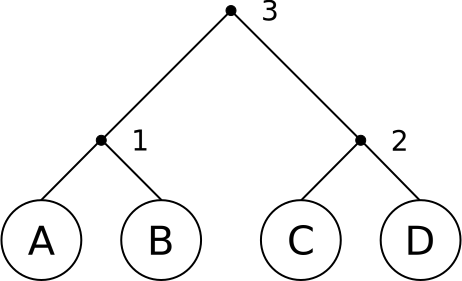
\includegraphics[scale=0.4]{img/tree_for_raam}
	\caption{A sample graph that can be processed using RAAM}
	\label{fig:tree_for_raam}
\end{center}
\end{figure}

\begin{figure}
\begin{center}
	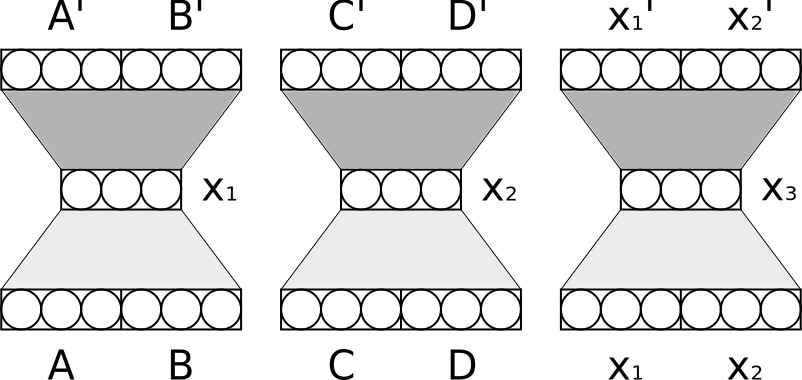
\includegraphics[scale=0.4]{img/raam1-3}
	\caption{Training set for the sample graph}
	\label{fig:raam1-3}
\end{center}
\end{figure}

\begin{figure}
\begin{center}
	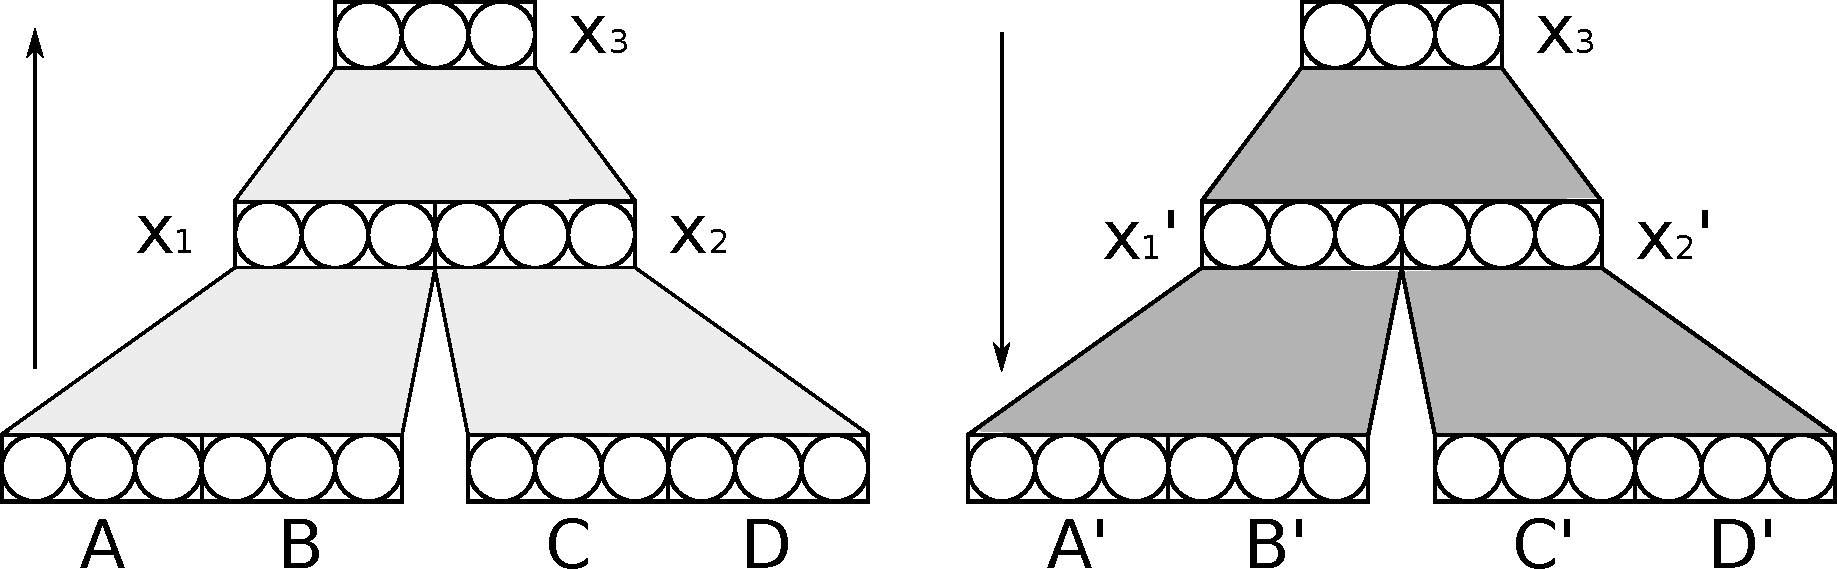
\includegraphics[scale=0.45]{img/raam_enc_dec}
	\caption{Graph compression and reconstruction using a trained RAAM model}
	\label{fig:raam_enc_dec}
\end{center}
\end{figure}

\newpage

\section{Training RAAM using SBLLM}
A RAAM model can be trained using simple backpropagation performed over the whole training set (Fig.~\ref{fig:raam1-3}) or using the \emph{encoding network}~\cite{goulon2005hopfield}. If the first method is used, the training can require hundreds to thousands iterations~\cite{sperduti1994labelling} and is vulnerable to the \emph{moving target} problem~\cite{pollack1990recursive}. The moving target problem can be avoided by using the encoding network approach, however, at the cost of introducing a more complex network model. In this paper a novel combination of the SBLLM with the RAAM model is evaluated. The main concern of this work was: would the SBLLM sufficiently adjust the network weights of both layers to provide a precise RAAM compressor and reconstructor. A high precision was crucial, as both these units are used to recursively process data - if an error is introduced at $i$th tree node, all subsequent nodes representations reconstructed from this node will become highly distorted and finally unrecognisable.

For evaluation, the syntactic trees dataset was used, which was described in the original article about the RAAM model~\cite{pollack1990recursive}. The dataset consists of 15 well formed syntactic trees representing sentences. Each sample consists of terminals D, A, N, V and P which stand for \emph{determiner}, \emph{adjective}, \emph{noun}, \emph{verb} and \emph{preposition}, respectively. Each terminal was represented as a 1-bit-in-5 code padded with 5 zeros. Each sample belongs to a phrase type and the correct clustering, reflecting the phrase types was one of the goals of the experiment. The sample, together with their ids (used later on) and phrase types are presented in Table~\ref{tab:syntax}.

\begin{table}[h!]
	\begin{center}
	\begin{tabular}{llll}
	\toprule
	phrase type & \# & structure \\
	\midrule
	NP & 1 & (D N)\\
	NP & 2 & (D (A (A (A N))))\\
	NP & 3 & (D (A N))\\
	NP & 4 & ((D N) (P (D N)))\\
	\midrule
	VP & 5 & (V (P (D N)))\\
	VP & 6 & (V (D (A N)))\\
	VP & 7 & (V (D N))\\
	\midrule
	PP & 8 & (P (D N))\\
	PP & 9 & (P (D (A N)))\\
	\midrule
	AP & 10 & (A N)\\
	AP & 11 & (A (A N))\\
	AP & 12 & (A (A (A N)))\\
	\midrule
	S & 13 & ((D N) V)\\
	S & 14 & ((D N) (V (D (A N))))\\
	S & 15 & ((D (A N)) (V (P (D N))))\\
	\bottomrule
	\end{tabular}
	\caption{Syntax trees}
	\label{tab:syntax}
	\end{center}
\end{table}


A RAAM model structure with 20 inputs, 10 hidden neurons and 20 output neurons was used, as in the case of the original experiment. The activation function was \emph{tanh} for the hidden layer and linear for the output layer. During the experiment, 50 RAAM networks were trained to learn the representations of the 15 syntactic trees and the best RAAM was selected as the one which achieved the smallest maximum reconstruction error of a single terminal representation amongst all the reconstructed trees, summed over all bits. The networks were trained for 5 iterations. The evolution of the maximum reconstruction error of the best network is presented in Fig.~\ref{fig:raam_syntax_best_mindiff}. It can be seen that out of 5 iterations only the first 4 resulted in a significant error decrease. The final bit error (without summing over bits) had the mean equal to $0.0390$, with standard deviation equal to $0.0880$. Four bits out of total 580 (0.7\%) had an error greater or equal to $0.5$, which made them unrecognisable. From all the reconstructed bits, 32 (5\%) had an error greater than $0.2$ which was the maximum error value used in the original article (denoted as $\tau$). The moving target problem didn't appear during the training.

\begin{figure}[h!]
\begin{center}
	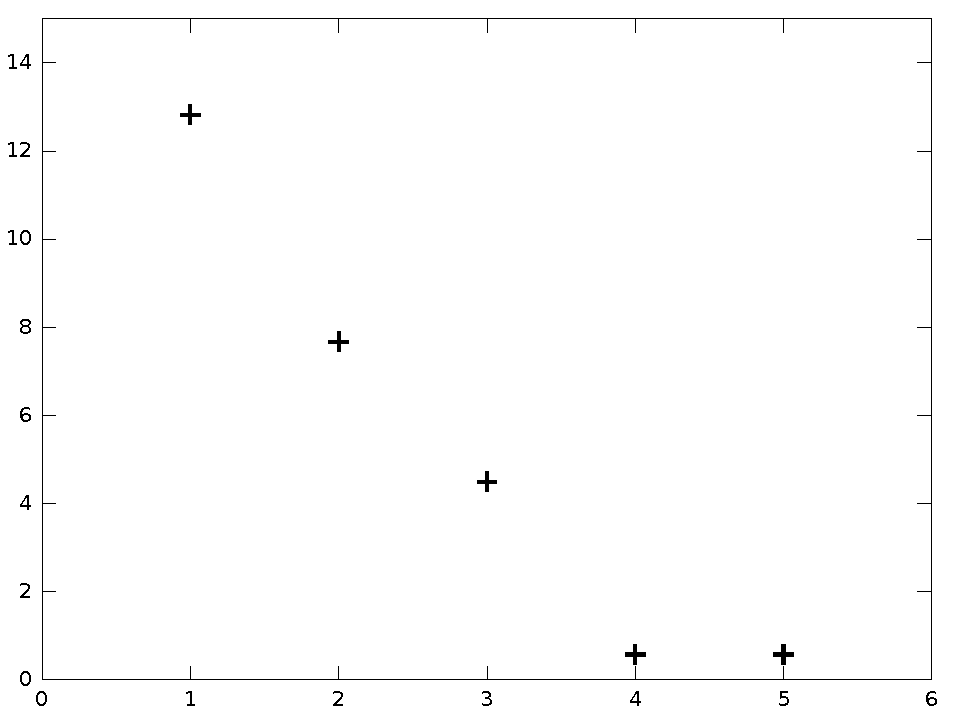
\includegraphics[scale=0.6]{img/raam_syntax_best_mindiff}
	\caption{Reconstruction error for training iterations 1 to 5 for the best RAAM model}
	\label{fig:raam_syntax_best_mindiff}
\end{center}
\end{figure}

To evaluate the ability of the obtained model to build meaningful representations, hierarchical clustering was performed on the obtained trees representations. The results are presented in Fig.~\ref{fig:raam_tree}. It can be seen that the syntactic trees are clustered according to their phrase types. Only the samples number 4, 8 and 9 were incorrectly attributed, which gives the same number of errors as in the original article (in which samples number 1, 4 and 10 were incorrectly attributed). The AP and VP clusters were matched perfectly.


\begin{figure}[h!]
\begin{center}
	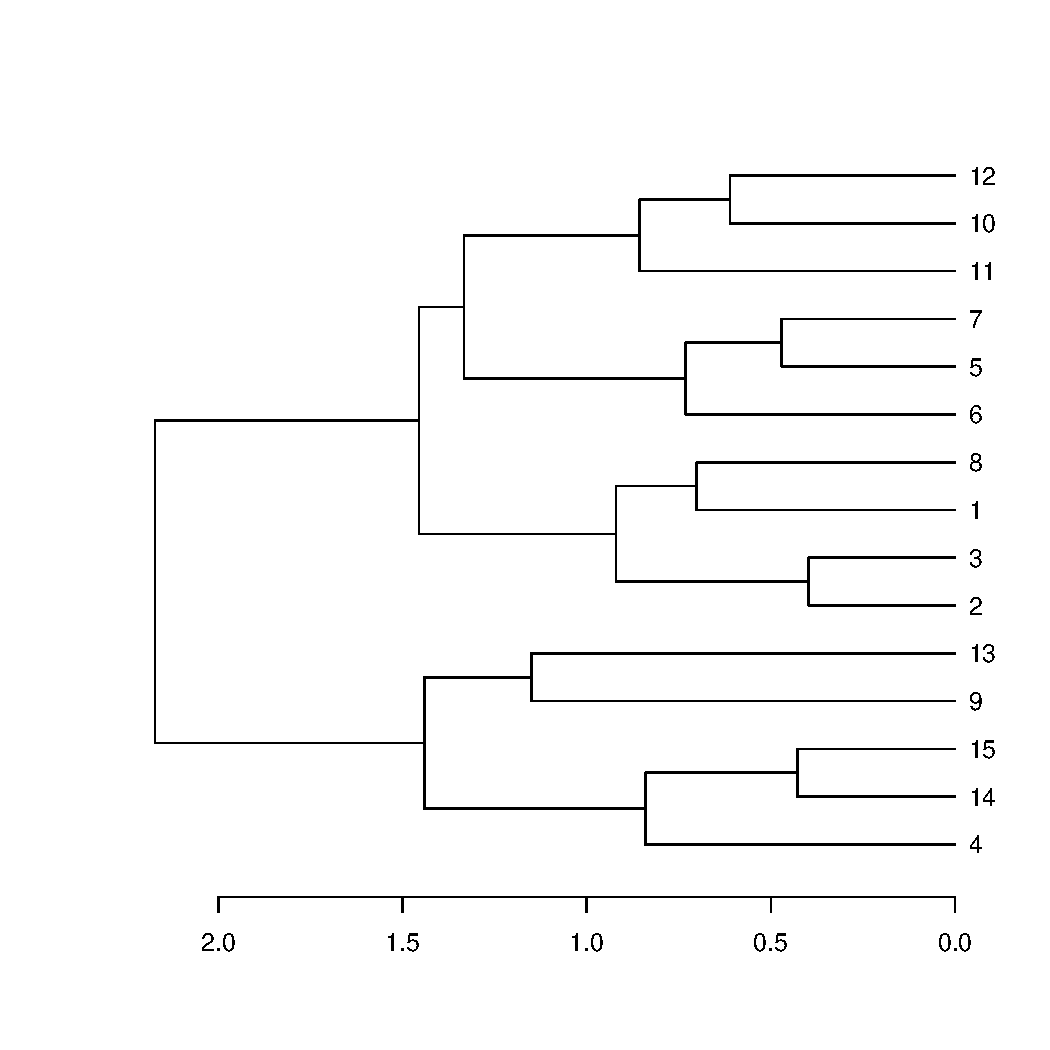
\includegraphics[scale=0.7]{img/raam-sbllm-syntax}
	\caption{Clustering results for the best RAAM model}
	\label{fig:raam_tree}
\end{center}
\end{figure}

\section{Conclusion}
The proposed combination of SBLLM and RAAM resulted in a model that can be trained in a very small number of epochs. Although the reconstruction precision of the obtained model was slightly worse than the precision of the model trained with standard backpropagation, the overall results were adequate for the task. The obtained model was able to build meaningful representations of the processed dataset, comparable to the results presented in the original article. Moreover, the training process wasn't affected by the \emph{moving target} problem, showing that such property can be achieved without imposing any additional constraints on the learning process and without the additional complexity of the \emph{encoding network} approach.

The presented model can be used for processing all the datasets that can be processed with the standard RAAM model. It should be also applicable to the more powerful LRAAM model, as only slight modifications would have to be made to process node labels at each node. The extension of the presented model to RAAM networks with more than three hidden layers seems, however, to be problematic, as the SBLLM is applicable to three-layer networks only and a new sensitivity-based model would have to be devised to take into account a larger number of layers.

%%%%%%%%%%%%%%%%%%%%%%%%%%%%%%%%%%%%%%%%%%%%%%%%%%%%%%%%%%%%%
%%%%% References %%%%%

\bibliography{bib/gnn,bib/fnn,bib/sensitivity}
\bibliographystyle{spiebib}   %>>>> makes bibtex use spiebib.bst

\end{document} 
